\linespread{1.5}
Considere um bola de futebol movimentando-se sob a ação da gravidade e da resistência do ar, conforme o diagrama abaixo.

\begin{figure}[H]
    \centering
    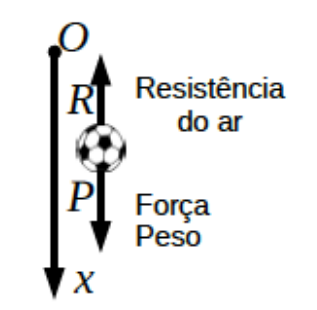
\includegraphics[width = 0.3\linewidth]{fig/edo43.png}
\end{figure}

O movimento da bola é descrito pela funções x(t) e a primeira e a segunda derivada dessa função representam a velocidade e a aceleração da bola, respectivamente. Para determinar o movimento da bola, utiliza-se a 2ª lei de Newton:
\begin{center}
    \textit{Massa $\times$ Aceleração = Soma das Forças Aplicadas}
\end{center}

que matematicamente pode ser traduzido como:
\begin{equation}
    \label{eq:edo431}
    m\ddot{x} = mg - \lambda \dot{x}
\end{equation}

a qual é uma E.D.O. linear não-homogênea, onde \textit{m} é a massa da bola, \textit{g} é a aceleração da gravitacional e $\lambda>0$ é a constante de resistência viscosa da bola em relação ao ar. Mesmo sem resolver a E.D.O. (\ref{eq:edo431}), é fácil ver que à medida em que a bola cai, sua velocidade aumenta, o que causa aumento da resistência do ar, até que a força peso seja neutralizada e a bola passe a se mover com velocidade constante, chamada velocidade terminal, dada por:
\begin{equation}
    v_T = \frac{mg}{\lambda}
\end{equation}

Com informações apresenta acima, pede-se:
\begin{itemize}
    \item[\textbf{a)}] Obtenha a solução geral da E.D.O. \ref{eq:edo431};
    \item[\textbf{b)}] Obtenha a solução particular que satisfaz as condições iniciais $x(0) = 0$ (posição inicial) e $\dot{x}(0) = 0$ (velocidade inicial);
    \item[\textbf{c)}] Sabendo que a bola tem velocidade terminal igual a 25 m/s e supondo que a mesma é solta do alto de uma torre com 100 m de altura, use o resultado obtido em \textbf{b)} para calcular que distância a bola cairia em 4 segundos. Compare com a distância de queda se não houvesse resistência do ar.
\end{itemize}